\appendix

\section{Attention Distribution Visualizations}
\label{app:attn_dist}

Figures~\ref{fig:attn_dist_0}--\ref{fig:attn_dist_199} show attention weight distributions at training steps 0, 49, 99, 149, and 199 from the h-e1 calibration experiment, illustrating how attention patterns evolve across evaluation examples.

\begin{figure}[h]
\centering
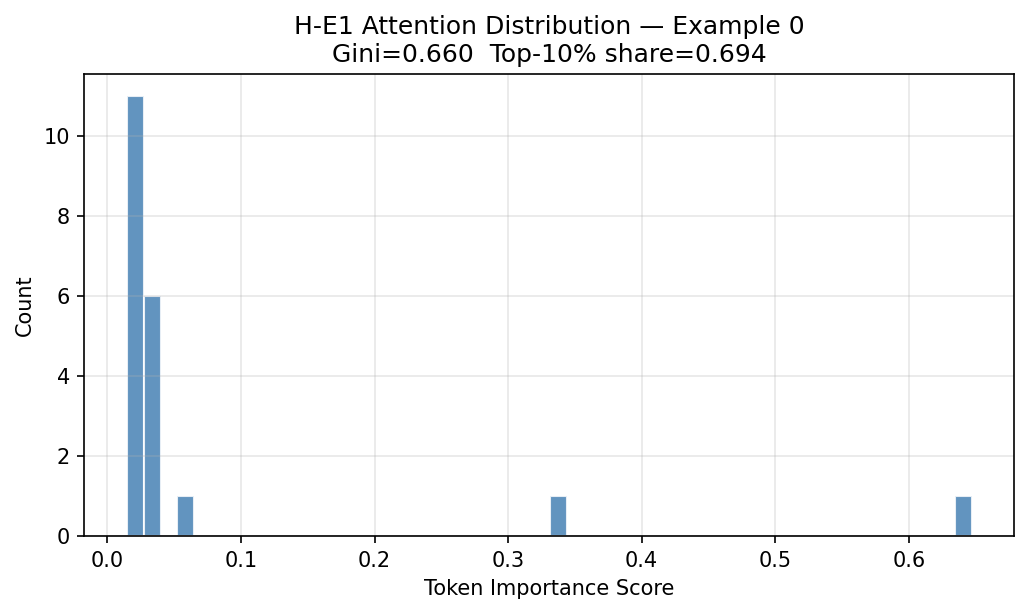
\includegraphics[width=0.45\textwidth]{figures/h_e1_attn_dist_0.png}
\caption{Attention distribution at evaluation example 0.}
\label{fig:attn_dist_0}
\end{figure}

\begin{figure}[h]
\centering
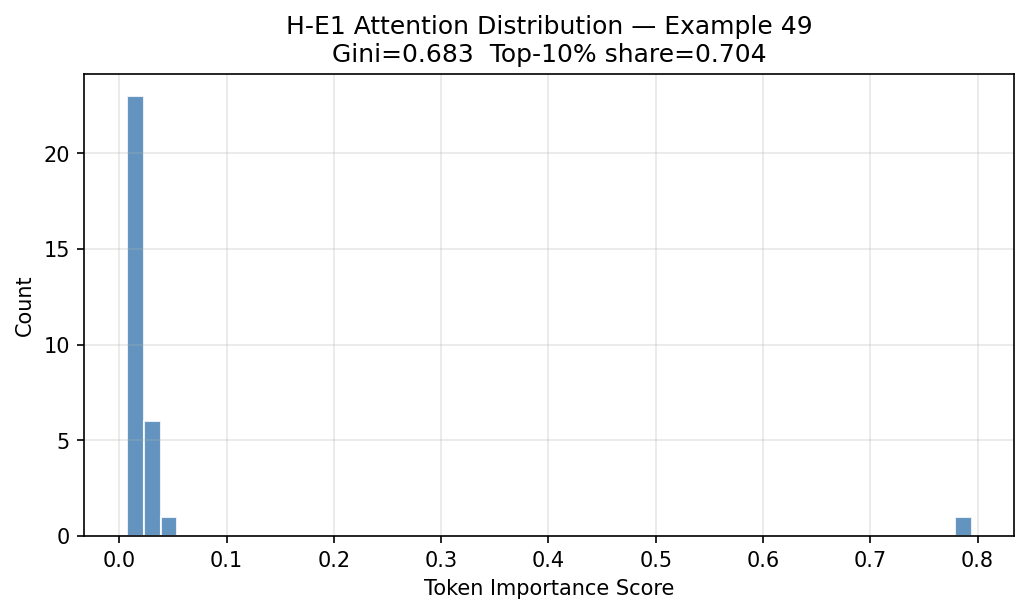
\includegraphics[width=0.45\textwidth]{figures/h_e1_attn_dist_49.png}
\caption{Attention distribution at evaluation example 49.}
\label{fig:attn_dist_49}
\end{figure}

\begin{figure}[h]
\centering
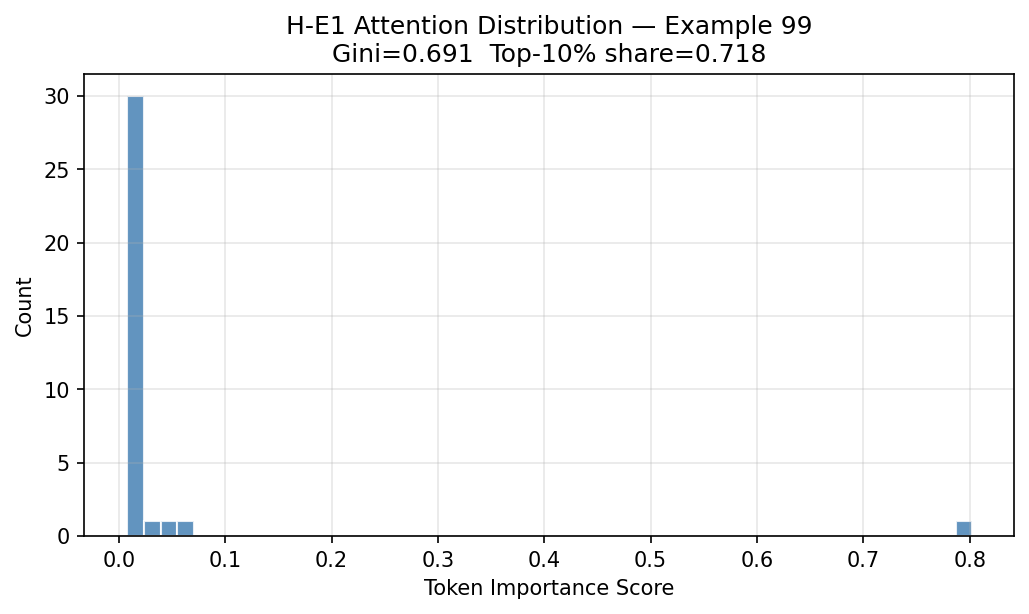
\includegraphics[width=0.45\textwidth]{figures/h_e1_attn_dist_99.png}
\caption{Attention distribution at evaluation example 99.}
\label{fig:attn_dist_99}
\end{figure}

\begin{figure}[h]
\centering
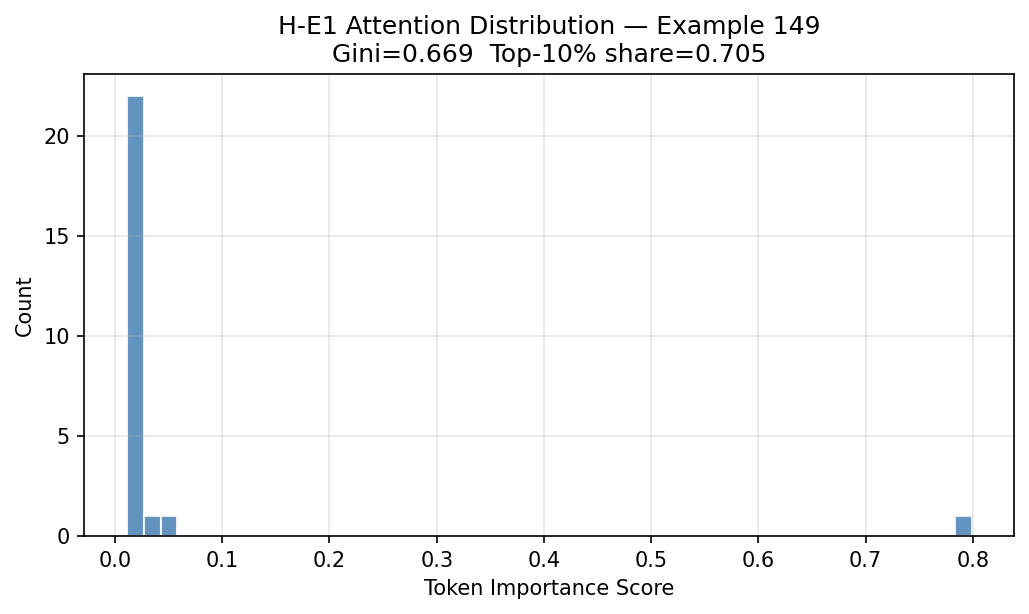
\includegraphics[width=0.45\textwidth]{figures/h_e1_attn_dist_149.png}
\caption{Attention distribution at evaluation example 149.}
\label{fig:attn_dist_149}
\end{figure}

\begin{figure}[h]
\centering
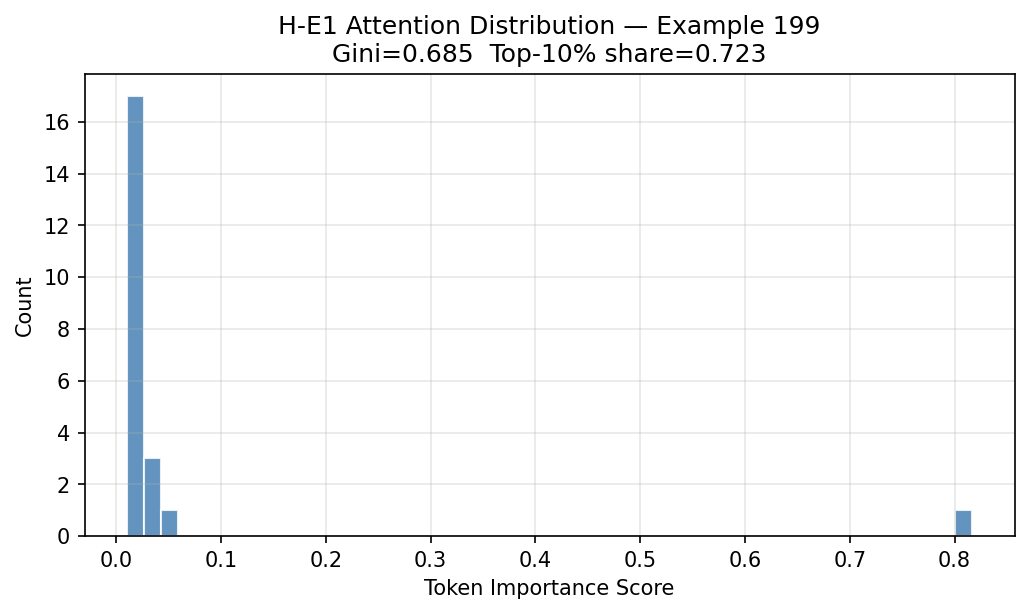
\includegraphics[width=0.45\textwidth]{figures/h_e1_attn_dist_199.png}
\caption{Attention distribution at evaluation example 199.}
\label{fig:attn_dist_199}
\end{figure}
